\chapter{Detektor}\label{chap:TheoDet}
Der Detektor läuft in zwei Schritten ab. Zuerst wird das Programm 
durchlaufen. Dabei wird ein Trace aufgezeichnet, welche die relevanten 
Informationen über den Programmablauf aufzeichnet. Dieser 
Trace wird im Anschluss analysiert, um Informationen über Probleme 
in dem Programm zu erhalten. Das Ganze wird gegebenenfalls mehrfach wiederholt,
um eine breitere Abdeckung des Programmcodes zu erreichen.


\section{Trace}\label{chap:background-sec:trace}
Um ein Program analysieren zu können, wird der Ablauf eines Programmdurchlaufs
(Trace) aufgezeichnet. Der grundlegende Aufbau des Trace basiert auf~\cite{PPDP18}. 
Er wird aber um Informationen 
über Locks erweitert. Der Trace wird für jede Routine
separat aufgezeichnet. Außerdem wird, anders als in~\cite{PPDP18} ein globaler
Program-Counter für alle Routinen und nicht ein separater Counter für jede 
Routine verwendet. Dies ermöglicht es, bessere Rückschlüsse über den genauen 
Ablauf des Programms zu erziehen.
Die Syntax des Traces in EBNF gibt sich 
folgendermaßen:
\begin{align*}
  \begin{matrix*}[l]
    T & = & ''\ [\ '',\ \{\ U\ \},\ ''\ ]\ ''; & \text{Trace}\\
    U & = & ''\ [\ '',\ \{\ t\ \},\ ''\ ]\ ''; & \text{lokaler Trace} \\
    t & = & signal(t, i)\ |\ wait(t, i)\ |\ pre(t, as)\ |\ post(t, i, x!) & \text{Event}\\
      &   & |\ post(t, i, x?, t') |\ post(t, default)\ 
      |\ close(t, x)\  
      & \\
      &   & |\ lock(t, y, b, c) |\ unlock(t, y); & \\
    a & = & x,\ (''\ !\ ''\ |\ ''\ ?\ ''); & \\
    as & = & a\ |\ (\{\ a\ \}, [\ ''\ default\ ''\ ]); & \\
    b & = & ''-''\ |\ ''t''\ |\ ''r''\ |\ ''tr'' & \\
    c & = & ''0''\ |\ ''1''
  \end{matrix*}
\end{align*}
wobei $i$ die Id einer Routine, $t$ einen globalen Zeitstempel, $x$ die Id eines 
Channels und $y$ die Id eines Locks darstellt. Die Events haben dabei folgende Bedeutung:
\begin{itemize}
  \item \texttt{signal(t, i)}: In der momentanen Routine wurde
    eine Fork-Operation ausgeführt,
    d.h. eine neue Routine mit Id $i$ wurde erzeugt.
  \item \texttt{wait(t, i)}: Die momentane Routine mit Id $i$ wurde soeben erzeugt. Dies ist 
    in allen Routinen außer der Main-Routine das erste Event in ihrem lokalen Trace.
  \item \texttt{pre(t, as)}: Die Routine ist an einer Send- oder Receive-Operation eines 
    Channels oder an einem Select-Statement angekommen, dieses wurde aber noch nicht 
    ausgeführt. Das Argument $as$ gibt dabei die Richtung und den Channel an. 
    Ist $as = x!$, dann befindet sich der Trace vor einer Send-Operation, bei 
    $as = x?$ vor einer Receive-Operation. Bei einem Select-Statement ist 
    $as$ eine Liste aller Channels für die es einen 
    Case in dem Statement gibt. Besitzt das Statement einen Default-Case, wird
    dieser ebenfalls in diese List aufgenommen.
  \item \texttt{post(t, i, x!)}: Dieses Event wird in dem Trace gespeichert, nachdem 
    eine Send-Operation auf $x$ erfolgreich abgeschlossen wurde. 
    $i$ gibt dabei die Id der sendenden Routine an.
  \item \texttt{post(t, i, x?, t')}: Dieses Event wird in dem Trace gespeichert, nachdem 
    eine Receive-Operation des Channels $x$ erfolgreich abgeschlossen wurde. 
    $i$ gibt dabei die Id der sendenden Routine an. $t'$ gibt den Zeitstempel an,
    welcher bei dem Pre-Event der sendenden Routine galt. Durch die Speicherung der Id und des 
    Zeitstempels der sendenden Routine bei einer Receive-Operation lassen sich 
    die Send- und Receive-Operationen eindeutig zueinander zuordnen.
  \item \texttt{post(t, default)}: Wird in einem Select-Statement der Default-Case ausgeführt,
    wird dies in dem Trace der entsprechenden Routine durch $post(t, default)$ 
    gespeichert.
  \item \texttt{close(t, x)}: Mit diesem Eintrag wird das schließen eines Channels $x$ 
    in dem Trace aufgezeichnet.
  \item \texttt{lock(t, y, b, c)}: Der Beanspruchungsversuch eines Locks mit id $y$ wurde gestartet. 
    $b$ gibt dabei die Art der Beanspruchung an. Bei $b = r$ war es eine R-Lock
    Operation, bei $b = t$ eine Try-Lock Operation und bei $b = tr$ ein Try-R-Lock
    Operation. Bei einer normalen Lock-Operation ist $b = -$. Bei einer 
    Try-Lock Operation kann es passieren, dass die Operation beendet wird, 
    ohne das das Lock gehalten wird. In diesem Fall wird $c$ auf $0$, und 
    sonst auf $1$ gesetzt. Das Trace-Element wird vor der abgeschlossen 
    Beanspruchung in den Trace eingefügt um sicher zu stellen, dass 
    ein zyklisches Locking auch dann erkannt wird, wenn es zu einem 
    tatsächlichen Deadlock führt. 
  \item \texttt{unlock(t, y)}: Das Lock mit id $y$ wurde zum Zeitpunkt 
    $t$ wieder freigegeben. 
\end{itemize}


Man betrachte als Beispiel das Programm in Abb.~\ref{Chap:Tracer-Sec:Trace-Fig:Example}.\\
\begin{figure}[h]
  \lstinputlisting{code/example_code_pre.txt}
  \caption{Beispielprogramm für Tracer}
  \label{Chap:Tracer-Sec:Trace-Fig:Example}
\end{figure}
Dabei ergibt sich der folgende Trace:
\begin{align*}
  [&[signal(1, 2),\ signal(2, 3),\ signal(3, 4),\ pre(4, a?, default),\ post(5, default)]\\
  &[wait(8, 2),\ lock(9, 1, -, 1),\ pre(10, x!),\ post(16, 2, x!),\ unlock(17, 1)]\\
  &[wait(11, 3),\ pre(12, y!),\ post(13, 3, y!),\ pre(14, x?),\ post(15, 2, x?, 10)]\\
  &[wait(6, 4),\ pre(7, y?),\ post(18, 3, y?, 12)]]
\end{align*}
Aus diesem Trace lässt sich der relevante Ablauf des Programms vollständig rekonstruieren.

\section{Analyze}
Nach dem das Programm durchlaufen und der Trace aufgezeichnet wurde, 
wird dieser anschließend analysiert. Dabei werden für die Erkennung von 
Problemen mit Mutexen und Channels zwei verschiedene Ansätze verwendet.

\subsection{Mutexe}
Man betrachte zuerst die Erkennung von zyklischem Locking. 
Da solche Situationen nur in ganz besonderen Situation auftreten 
(in Abb.~\ref{Chap:Analyze-Sec:Mutex-Fig:Zyclic} müssen Zeilen 
7 und 14 genau gleichzeitig ausgeführt werden, ohne dass Zeile 8 oder 15 ausgeführt werden), muss 
ein Detektor, welcher vor solchen Situationen warnen soll, nicht nur tatsächliche Deadlocks, sondern
vor allem potenzielle, also nicht tatsächlich aufgetretene Deadlocks erkennen. Die Erkennung der 
potenziellen Deadlocks basiert hierbei auf iGoodLock~\cite{iGoodLock} und UNDEAD~\cite{Undead}. 
Dabei wird für jede Routine ein Lock-Baum aufgebaut. Jeder in der Routine vorkommende 
(RW-)Mutex $m_i$ wird durch einen Knoten $k_i$ in dem Baum repräsentiert. 
In diesem Baum gibt es nun eine gerichtete Kante von $k_1$ nach $k_2$, wenn 
$m_1$ das
von der Routine momentan gehaltene Lock ist, welches zuletzt von der Routine 
geschlossen worden ist, währen das Lock $m_2$ geschlossen wird~\cite{lock-tree}.
Ist es nun möglich, Knoten aus verschiedenen Bäumen, welche den selben
Mutex repräsentieren so zu verbinden, dass der entstehende Graph einen Zyklus 
enthält, bedeutet dies, dass in dem Programm zyklisches Locking möglich ist. 
Man betrachte dazu das Programm in Abb.~\ref{Chap:Analyze-Sec:Mutex-Fig:ZyclicTreeCode}
\begin{figure}[h!]
  \lstinputlisting{code/example-lock-tree-code.txt}
  \caption{Beispielprogramm zyklisches Locking}
  \label{Chap:Analyze-Sec:Mutex-Fig:ZyclicTreeCode}
\end{figure}
In Abb.~\ref{Chap:Analyze-Sec:Mutex-Fig:ZyclicTreeImg} sind die entsprechenden
Lock-Bäume, sowie der enthaltene Zyklus graphisch dargestellt. Es sei allerdings 
festzuhalten, dass besonders bei der Verwendung von RW-Locks, nicht jeder 
Zyklus auch direkt zu einem potenziellen Deadlock führen kann. Wie solche 
False-Positives verhinder werden können, wird in dem Abschnitt zur Implementierung
des Detektors (Abs.~\ref{Chap:Implement-Sec:Mutex}) noch genauer betrachtet.

\begin{figure}[h!]
  \centering
  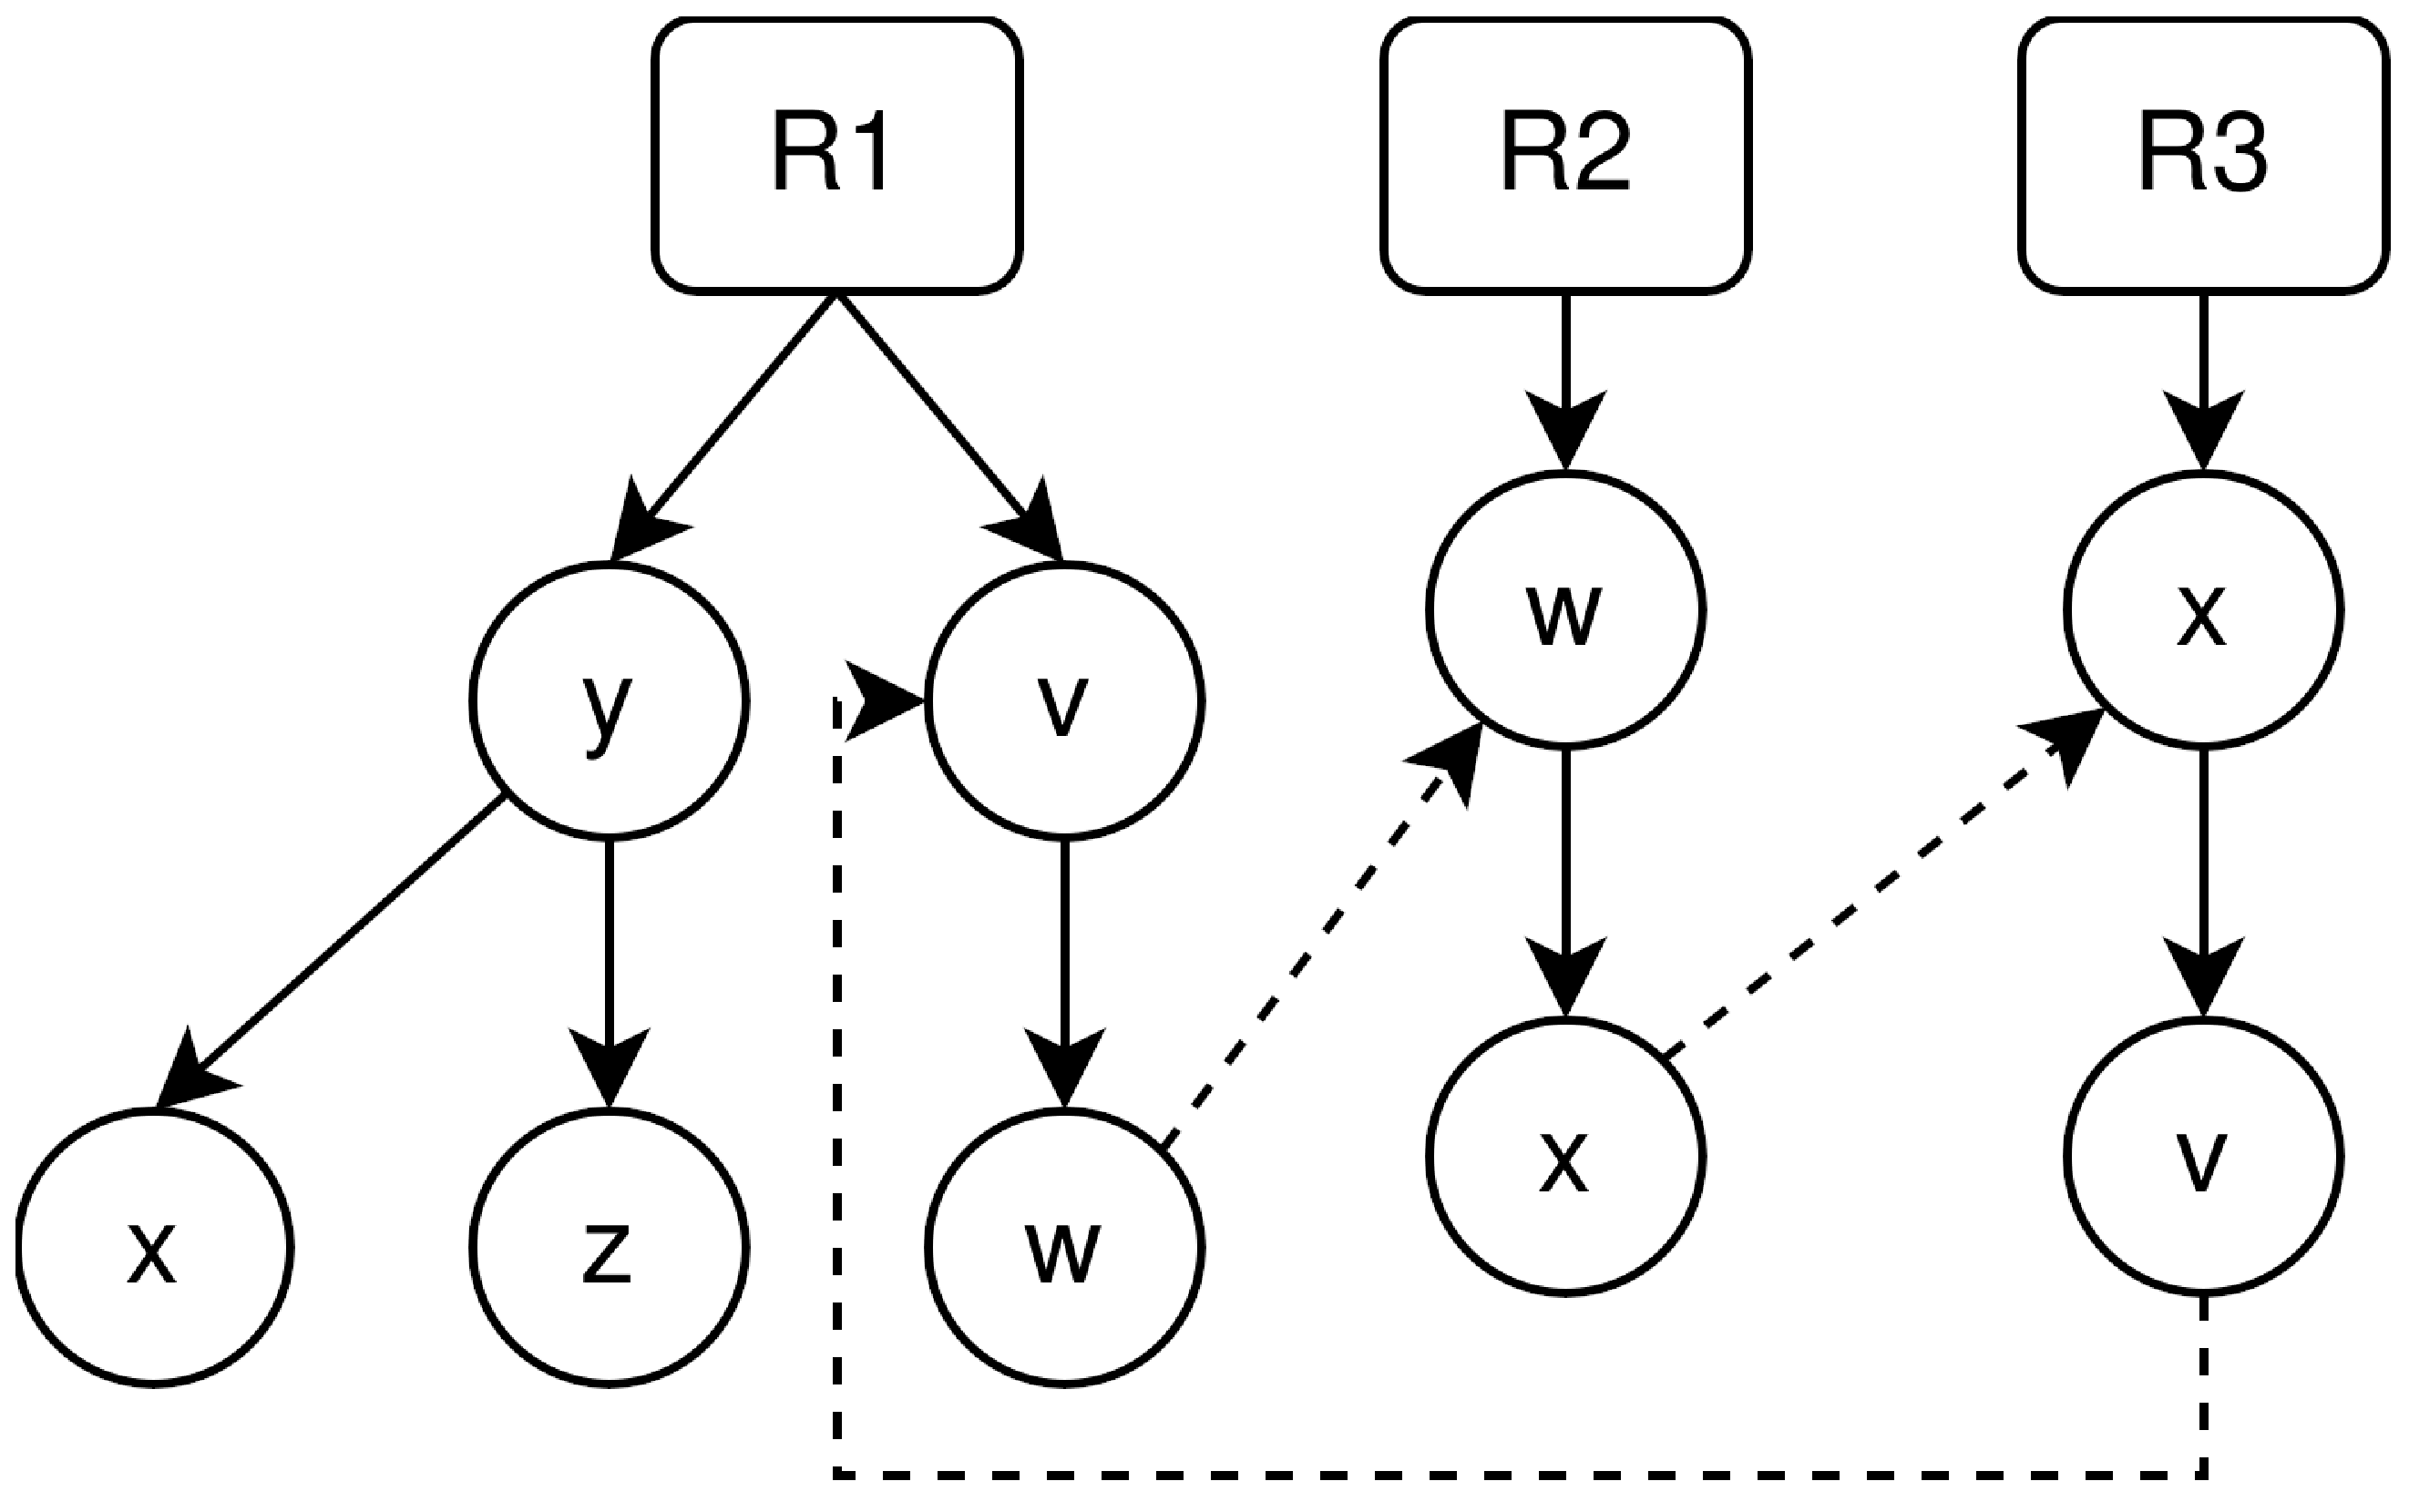
\includegraphics[width=0.5\textwidth]{img/tree_example.eps}
  \caption{Graphische Darstellung des Lock-Graphen für das Beispielprogramm in 
    Abb.~\ref{Chap:Analyze-Sec:Mutex-Fig:ZyclicTreeCode}. Durch die gestrichelten 
    Pfeile wird der enthaltenen Zyklus angezeigt.}
    \label{Chap:Analyze-Sec:Mutex-Fig:ZyclicTreeImg}
\end{figure}
Doppeltes Locking kann, anders als das zyklische Locking nur erkannt werden, 
wenn es tatsächlich auftritt. Dazu wird überprüft, ob es in einem Trace 
für eine der Routinen ein Paar von Lock-Elementen des selben Mutex gibt, 
ohne dass es zwischen den beiden ein Unlock-Element des Mutex gibt. 
Hierbei muss außerdem gelten, dass es sich nicht bei beiden Lock-Operationen 
um RLocks handelt und das die spätere Lock-Operation keine TryLock-Operation ist.  



\subsection{Channel}\label{Chap:Theo-Sec:Analyze-SubSec:Channel}
Man möchte nun Situationen auf Channels erkennen, in welchen eine 
Routine versucht eine Nachricht zu versenden oder zu empfangen, es aber 
keinen möglichen Kommunikationspartner gibt. Für ungebufferte 
Channels, sowie in manchen Fällen bei gebufferten Channels kann dies zu einer 
blockade der entsprechenden Routine führen. Befindet sich die Situation in 
der Main-Routine, dann kann es dazu führen, dass das gesamte Programm 
nicht terminieren kann. In Fällen wie z.B. in 
Abb.~\ref{Chap:Analyze-Sec:Channel-SubSec:Dangling-Fig:ExDanglingWithout}, 
\begin{figure}[h!]
  \lstinputlisting{code/example-dangling-without.txt}
  \caption{Hängender Channel ohne Deadlock}
  \label{Chap:Analyze-Sec:Channel-SubSec:Dangling-Fig:ExDanglingWithout}
\end{figure}
in welcher eine Nicht-Main-Routine blockiert (das Receive auf \texttt{x} findet 
keinen Send-Partner) wird die entsprechende Routine bei der Terminierung 
der Main-Routine automatisch abgebrochen. Man bezeichne einen solchen Fall 
als hängende Routine. Mit gebufferten Channels kann es passieren, 
das eine Send-Operation zwar erfolgreich ausgeführt wird, die entsprechende
Nachricht aber nie ausgelesen wird.

Um solche Situationen zu erkennen werden alle möglichen Paare von Kommunikationspartner
betrachtet, und dabei überprüft, ob diese Zuordnung zu Send- oder Receive-Operationen führt, 
welche keine möglichen Partner besitzen. Dabei sei zu beachten, dass nur weil eine Send- und eine 
Receive-Operation auf dem selben Channel geschehen, nicht 
in jedem Fall eine Kommunikation zwischen diesen möglich ist. Man betrachte dazu das Beispiel in 
Abb.~\ref{Chap:Analyze-Sec:Channel-SubSec:Dangling-Fig:NoSync}.
\begin{figure}[h!]
  \lstinputlisting{code/example-no-sync.txt}
  \caption{Beispielprogramm für unmögliche Synchronisation}
  \label{Chap:Analyze-Sec:Channel-SubSec:Dangling-Fig:NoSync}
\end{figure}
Auf dem Channel \texttt{x} wird in 1 gesendet und kann in 2 und 3 empfangen werden. Da es zwei Receive, 
aber nur eine Send-Operation gibt, kommt es zu einem hängenden Channel. Betrachtet man nur 
Channel \texttt{x} könnte man davon ausgehen, dass 1 nach 2 senden kann. 
Dies ist aber nicht möglich. Da der Channel \texttt{y} in 1 nach \texttt{x} sendet, 
in 2 allerdings von \texttt{x} empfangen muss, ist eine Synchronisierung auf \texttt{x} von 1 nach 
2 nicht möglich. Die beiden Operationen bilden demnach keine möglichen Kommunikationspartner.

Um mögliche Kommunikationspartner zu erkennen, nicht mögliche Kommunikationspartner wie in 
Abb.~\ref{Chap:Analyze-Sec:Channel-SubSec:Dangling-Fig:NoSync} aber auszuschließen, werden
Vector-Clocks verwendet.\\
In einem ersten Durchlauf wird dabei der Trace mit Vector-Clock Informationen nach der Methode 
von Fidge~\cite{Fidge} erweitert. Für jede Routine 
wird eine Vector-Clock gespeichert, welche für jede Routine einen Wert enthält. Zu Begin werden 
all diese Werte auf 0 gesetzt. Bei jedem Post-Event, sowohl für Send als auch Receive und für 
Signal und Wait Elemente wird der Wert der eigenen Routine in der lokalen Vector-Clock um eins 
erhöht. Bei einem Post-Receive und einem Wait Element wird die Vectorclock $vc'$ betrachtet, 
welche in der sendenden Routine zum Zeitpunkt des Post-Send- bzw. Signal-Elements vorlag. 
Da ein Send- bzw. Signal-Event immer vor dem Receive- bzw. Wait-Element erzeugt wird, wurde 
die entsprechende Vectorclock in jedem Fall bereits bestimmt. Die Zuordnung der Trace-Elemente 
ist möglich, da der globale Counter bei einem Send an den Empfangenden Channel mitgesendet 
wird, und in dem entsprechenden Post-Receive-Element gespeichert wird.
Bei einem Select-Statement wird nur derjenige Fall betrachtet, der auch tatsächlich ausgeführt wurde.
Diese Send-Vector-Clock \texttt{vc'}
wird nun mit der lokalen Vector-Clock \texttt{vc} der empfangenden Routine, bzw. der Wait-Routine 
\texttt{q} verrechnet und ersetzt diese. Dabei gilt\\
\begin{figure}[h]
  \centering
  \lstinputlisting[frame=none, numbers=none, xleftmargin=0.3\textwidth, xrightmargin=0.3\textwidth]{code/vector-clock.txt}
\end{figure}\\
wobei $n$ die Anzahl der Routinen ist.\\
Für alle andern Elemente, z.B. Pre usw., wird einfach die lokale Vector-Clock der Routine übernommen, 
ohne diese zu verändern. Da nun die Vector-Clocks zu jedem Zeitpunk bestimmt wurde, kann jedem 
Send- und Receive-Trace-Element eine Pre- und eine Post-Vector-Clock zugeordnet werden. 
Dabei handelt es sich um die Vector-Clocks, die bei Erzeugung des Pre- bzw. Post-Events in 
der Routine, in der die Operation ausgeführt wurde vorlag. Für hängende Operationen, 
bei denen kein Post-Element existiert, werden alle Werte der Post-Vector-Clock auf 
max(Int32) gesetzt. Für Close gilt, 
dass die Pre-Vectorclock gleich der Post-Vectorclock ist. Andere Elemente 
werden in den VAT nicht aufgenommen, da sie 
für die anschließende Analyse nicht benötigt werden.

Basierend auf Vectorclocks gilt, dass $x$ ist eine Ursache von $y$ ist ($x < y$) wenn gilt, dass 
\begin{align}
  VC(x) < VC(y) \Leftrightarrow \forall z (VC(x)[z] \leq VC(y)[z]) \land \exists z' (VC(x)[{z'}] < VC(y)[{z'}]),
\end{align}
wobei $VC(x)[z]$ das $z$-te Element der Vectorclock von $x$ bezeichnet.
Man bezeichne $x$ und $y$ als unvergleichbar ($x \not\lessgtr y$), wenn 
$x \not< y $ und $y \not< x$.
Sind zwei Vector-Clocks 
unvergleichbar, sind sie unabhängig und die entsprechenden Operationen 
können somit gleichzeitig auftreten. 
Man erkennt also zwei Operationen, welche auf ungebufferten Channels eine mögliche Kommunikation durchführen 
können daran, dass sie auf dem selben Channel definiert sind, eine Send-
und eine Receive-Operation definieren und dass 
 ihre Pre- oder Post-Vector-Clocks unvergleichbar sind.\\
Um alternative Kommunikationspartner für Channel zu finden, werden also
die Pre- und Post-Vector-Clocks der VAT-Elemente mit dem selben Channel verglichen um
solche Paare zu finden.\\ Wenn sich eine Send- und Receive-Operation, 
welche bezüglich der Vector-Clocks zwar kommunizieren könnten so von Mutexen 
umschlossen werden, das die Operationen nicht gleichzeitig ausgeführt werden 
können, bilden sie keine gültige Kommunikation.


In gebufferten Channels ist nicht notwendig, dass Send und Receive gleichzeitig
ausgeführt werden.
\begin{figure}[h!]
  \centering
  \lstinputlisting{code/buffered_not_possible.txt}
  \caption{Beispielprogramm für unmögliche Synchronisation auf gebuffertem Channel}
  \label{Chap:Analyze-Sec:Channel-SubSec:Dangling-Fig:BufferedNoSync}
\end{figure}
Theoretisch ist es einem gebufferten Channel möglich bei einem Send mit 
jedem Receive auf dem selben Channel zu kommunizieren, welches nicht 
streng vor dem Send ausgeführt werden muss. In der Praxis geben sich allerdings 
Situationen in welchen eine Synchronisation zwischen Send- und Receive nicht 
möglich ist. Man betrachte dazu das Beispiel in 
Abb.~\ref{Chap:Analyze-Sec:Channel-SubSec:Dangling-Fig:BufferedNoSync}.
Auf den ersten Blick scheint es möglich, dass beide Send (1, 2) mit dem 
Receive kommunizieren könnten. Dies ist aber nicht der Fall.
Es ist klar ersichtlich, dass 1 von 2 ausgeführt wird. Da der Buffer von 
gebufferten Channels in der Praxis als FIFO-Queues funktionieren, 
bedeutet dies, dass in 3 in jedem Fall die Nachricht aus 1 empfangen wird.
Allgemein kann man sagen, dass das $n$-te Send mit dem $n$-ten Receive 
kommuniziert. 
Das 1 vor 2 ausgeführt 
werden muss ist aus den Vectorclocks ablesbar. Um zu überprüfen, 
ob eine Kommunikation möglich ist, werden daher für jede Send $s$ Operation 
die Anzahl der Send Operationen auf dem selben Channel bestimmt, welche streng vor $s_i$ 
ausgeführt werden ($\#s_{i, <}$) sowie die Anzahl der Operationen, welche nebenläufig mit $s_i$ 
ausgeführt werden ($\#s_{i, \not\lessgtr}$). Das selbe wird analog auch 
für jedes Receive $r_i$ ($\#r_{i, <}, \#r_{i, \not\lessgtr}$) bestimmt. 
Damit ein Send-Receive Paar $s_i - r_j$ auf 
einem gebufferten Channel nun basierend auf der FIFO-Queue möglich ist, 
also eine mögliche Kommunikation bilden muss gelten, dass 
\begin{align}
  \#s_{i, <} &\leq \#r_{j, <} + \#r_{i, \not\lessgtr}\label{Form:1}\\
  \#s_{i, <} + \#s_{i, \not\lessgtr} &\geq \#r_{j, <}\label{Form:2}
\end{align}
Die Motivation für diese Formeln wird klar, wenn man das Beispiel in 
Abb.~\ref{Chap:Analyze-Sec:Channel-SubSec:Dangling-Fig:BufferForm} betrachtet.
\begin{figure}[h!]
  \centering
  \lstinputlisting{code/buffered_form.txt}
  \caption{Beispielprogramm als Motivation für Formeln~(\ref{Form:1}) und~(\ref{Form:2})}
  \label{Chap:Analyze-Sec:Channel-SubSec:Dangling-Fig:BufferForm}
\end{figure}
Man suche nun nach möglichen Kommunikationspartnern für das Send in 2. 
Da der Buffer eines Channels in Go praktisch wie eine FIFO-queue implementiert
ist, ist es nicht möglich, dass 2 mit 5 kommuniziert, da dies das erste 
Receive ist, das Send in 1 aber vor dem in 2 ausgeführt wird. Dass diese 
Kommunikation nicht möglich ist, wird durch Formel~\ref{Form:1} sicher gestellt.
Auch die Kommunikation mit dem Receive in 8 ist nicht möglich. Nur die Send in 
1 und 4 können vor dem Send in 2 ausgeführt werden. Das bedeutet, das das 
Send in 2 maximal das 3. Send in dem Programm darstellt. Dies bedeutet, 
dass für einen möglicher Kommunikationspartner maximal 2 andere Receives vor dem 
möglichen Kommunikationspartner ausgeführt werden dürfen. Da 8 aber in jedem 
Fall das 4. Receive darstellt, ist eine Kommunikation zwischen 2 und 8 nicht mögliche.
Formel~\ref{Form:2} sorgt dafür, dass solche Paare nicht fälschlicherweise 
als Kommunikationspartner gesehen werden.

Nachdem nun alle möglichen Kommunikationspartner ermittelt wurden, 
können die möglichen Ausführungspfade betrachtet werden, um zu überprüfen, 
ob diese zu Problemen führen. Der Detektor geht dazu alle vorhandenen Send-Operationen 
durch und ordnet Schrittweise jeder Operation eine Receive-Operation zu, so dass 
die Send- und Receive-Operation potenzielle Kommunikationspartner 
bilde und keine zwei Send-Operationen die selbe Receive-Operation 
besitzen. Es kann nun vorkommen, dass ein Teil der Send-Operationen bereits eine 
Receive-Operation zugeordnet bekommen haben, einer weiteren Send-Operation 
aber kein gültiges Receive zugeordnet werden kann. Dies bedeutet, dass 
wenn der Ablauf des Programm wie in den bereits zugeordneten Paaren geschieht, die Operation, 
welcher keine gültige Receive-Operation zugeordnet werden kann, keinen 
gültigen Kommunikationspartner besitzt. Dies bedeutet, dass es zu einem 
blockierten Programm, einer hängenden Routine, oder einer nicht ausgelesenen Nachricht 
in einem gebufferten Channel kommt. In diesem Fall wird eine Warnung 
mit den entsprechenden Informationen ausgegeben. Das selbe wird auch umgekehrt durchgeführt. Es wird als 
versucht jeder Receive-Operation eine Send-Operation zuzuordnen. 
Auch hier führt eine Situation, in welcher keine gültige Zuordnung für eine der Operationen 
möglich ist zu einem Bug. \\
Nicht alle betrachteten Ordnungen bilden gültige Ordnungen. Da die Operationen 
innerhalb einer Routine sequenziell abgearbeitet werden ist eine Zuordnung nur 
dann gültig, wenn für jede Operation \texttt{p}, welche in der Ordnung 
betrachtet wird auch alle anderen Operationen in der selben Routine, welche 
vor \texttt{p} ausgeführt werden in der Zuordnung vorhanden sind.

Man betrachte als Beispiel das Programm in Abb.~\ref{Chap:Analyze-Sec:Channel-SubSec:Dangling-Fig:PorgVC}.
\begin{figure}[h!]
  \centering
  \lstinputlisting{code/example-vector-clock-prog.txt}
  \caption{Beispielprogramm für die Betrachtung der Vector-Clocks}
  \label{Chap:Analyze-Sec:Channel-SubSec:Dangling-Fig:PorgVC}
\end{figure}
Zuerst betrachte man den Fall, in dem 1 mit 4 und dann 3 mit 2 synchronisiert.
In diesem Fall erhält man folgenden Trace:
\begin{align*}
  [&[signal(1, 2), signal(2, 3), pre(3, 1?), post(9, 1, 1?, 6)]\\
  &[wait(5, 2), pre(6, 1!), post(7, 1, 1!), pre(8, 1?), post(12, 2, 1?, 10)]\\
  &[wait(4, 3), pre(10, 1!), post(11, 2, 1!)]]
\end{align*}
Bei diesem Ablauf besitzen alle Operationen einen gültigen 
Kommunikationspartner. Es tritt also kein Bug auf.
Aus diesem Trace lassen sich nun die Vector-Clocks für die einzelnen Operationen berechnen.
Der Ablauf des Programs, welcher dem Trace entspricht, inklusive der Vector-Clocks 
ist in Abb.~\ref{Chap:Analyze-Sec:Channel-SubSec:Dangling-Fig:VC} gegeben.
\begin{figure}[h!]
  \centering
  
\includegraphics[width=0.5\textwidth]{img/vc.eps}
  \caption{Ablaufdiagramm mit Vector-Clocks für das Beispiel in Abb.~\ref{Chap:Analyze-Sec:Channel-SubSec:Dangling-Fig:PorgVC}}
  \label{Chap:Analyze-Sec:Channel-SubSec:Dangling-Fig:VC}
\end{figure}
Von diesen lassen sich nun die Pre- und Post-Vector-Clocks direkt ablesen.
Für den Vectorclock-Annotierte-Trace (VAT) werden diese in der Form $^{vc}a^{vc'}$ 
mit der Pre-Vector-Clock $vc$ und der 
Post-Vector-Clock $vc'$ und der Channel-Operation $a$ angegeben.
Der VAT gibt sich in diesem Fall also als
\begin{align*}
  [&[^{[2,0,0]}x_4?^{[3,2,0]}]\\
  &[^{[1, 1, 0]}x_1!^{[1, 2, 0]}, ^{[1, 2, 0]}x_2?^{[2, 3, 2]}]\\
  &[^{[2, 0, 1]}x_3!^{[2, 0, 2]}]]
\end{align*}
Basierend auf den Vectorclocks wird nun klar, dass 1 mit 4 und 3 sowohl mit 
2 als auch 4 kommunizieren kann. Basierend darauf lassen sich nun für die 
von Send-Operationen ausgehenden Ordnungen die Kommunikationen als
  \begin{align*}
    x_1! &\to x_4?  \\
    x_3! &\to x_2?  
  \end{align*}
oder 
\begin{align*}
  x_3! &\to x_4?\\
  x_1! &\to \lightning
\end{align*}
und für die von Receive-Operationen ausgehenden Ordnungen als
  \begin{align*}
    x_4? &\leftarrow x_1!\\
    x_2? &\leftarrow x_3?
  \end{align*}
  oder 
  \begin{align*}
    x_4? &\leftarrow x_3?\\
    x_2? &\leftarrow \lightning
  \end{align*}
  bestimmen.
$\lightning$ bedeutet hierbei, das kein gültiger Kommunikationspartner möglich ist.
Bei ungebufferten Channels führen solche Situationen zu einer blockierenden Routine
oder gegebenenfalls sogar zur zu einer Blockades des gesamten Programms.
Bei gebufferten Channels führen sie entweder zu einer Blockade oder zumindest 
zu einer nie gelesenen Nachricht. All diese Fälle werden als Bug betrachtet
und werden somit von dem Detektor als potenzielle Bug angegeben.

Das betrachtete Beispiel zeigt gut den Vorteil der Verwendung von Vectorclocks.
Bei dem Durchlaufen des Programms sind keine Bugs aufgetreten. Dennoch 
ist es mit den Vectorclocks möglich alternative Kommunikationsabläufe 
zu betrachten und potenzielle Bugs in diesen zu finden.  

\subsection{Close}
Versuch ein Programm auf einem geschlossenen Channel zu senden kommt es zu einem Laufzeitfehler, 
welcher in einem Programmabbruch führt. Solch eine Situation lässt sich 
dadurch erkennen, dass eine Close- und eine Send-Operation auf dem selben Channel
gleichzeitig ablaufen können, dass also die Pre- oder Post-Vectorclock 
der Send-Operation unvergleichbar mit der Vectorclock der Close-Operation 
ist. Situationen, bei denen die Vectorclocks der Send-Operation streng später 
als die der Close-Operation sind führen immer dazu, das es zu einem einem 
Send auf einem geschlossenen Channel kommt. In diesem Fall kommt es also immer 
zu einem Laufzeitfehler des Programms, durch welchen das Programm abgebrochen wird.
Dies kann direkt, auch ohne die Betrachtung der Vectorclocks erkannt werden. 

\section{Select}\label{Chap:Back-Sec:Select}
In Go können Select-Statements dazu verwendet werden, abhängig davon, 
auf welchen Channels Nachrichten gesendet werden unterschiedliche Programmteile
auszuführen. Dies erschwert die Analyse des Programs, da der 
tatsächliche Programmablauf dabei praktisch nicht-deterministisch werden 
kann~\cite{select-spec}. Da der aufgezeichnete Trace immer nur einen 
Programmablauf betrachtet, führt dies zu Problemen, da 
nicht betrachtete Ausführungspfade zu Deadlocks oder anderen Problemen 
führen können. Eine Möglichkeit besteht darin, das Programm mehrfach auszuführen, 
und dabei immer unterschiedliche Select-Cases zu erzwingen. Ein solcher 
Ansatz wird unter anderem in GFuzz~\cite{gfuzz} verwendet. Dazu werden die 
Select-Statements in dem Programmcode so verändert, dass aus den vorhandenen 
Cases eines gezielt bevorzugt werden kann.
Der Ablauf eines Programms bezüglich seiner 
Select-Statements kann nun als Liste von Tupeln 
$[(s_0, c_0, e_0), \ldots, (s_n, c_n, e_n)]$ dargestellt werden. Dabei 
bezeichnet $s_i (0 \leq i \leq n)$ die ID einer Select-Operation, $c_i$ 
die Anzahl der Cases in dieser Operation und $e_n$ den Index des ausgeführten 
Case. Das Programm wird nun mehrfach durchlaufen, wobei die Ordnung zufällig 
verändert wird. Dazu wird nach jedem Durchlauf der Index $e_i$ jedes Tupels 
auf einen zufälligen, aber gültigen Wert gesetzt. Da die Anzahl der möglichen 
Ausführungspfade durch die Select-Statements gegebenenfalls gegen unendlich gehen kann,
ist es nicht möglich jede mögliche Kombination von Select-Cases auszuführen.
Aus diesem Grund sammelt GFuzz während der Ausführung einer Ordnung Informationen 
über diese, um die Qualität einer Ordnung abzuschätzen. Aus diesen wird 
eine Wertung für die durchlaufenden Ordnung bestimmt, über welche die 
Anzahl der Mutationen bestimmt werden. 

Die Betrachtung von verschiedenen Pfaden von Select wird auch für GoChan 
verwendet. Für jeden Durchlauf wird 
der Trace aufgezeichnet und dieser
analysiert. Die Auswahl der Pfade wird dabei vereinfacht. Anders als 
in GFuzz basieren die betrachteten Ausführungsordnungen nicht auf schon versuchten Ordnungen,
sondern es wird eine Menge von vollständig zufälligen Ordnungen betrachtet.
Die Sammlung von Informationen über die einzelnen Abläufe bedeutet einen 
deutlichen Mehraufwand, sowohl bei der Implementierung, als auch bei der eigentlichen 
Bestimmung der für die Abschätzung benötigten Werte. Da der Nutzen dabei eher gering ist,
wird darauf verzichtet.